% \clearpage
% \setcounter{page}{1}
% \maketitlesupplementary

\begin{center}
    \section*{------ Supplementary Material ------}
\end{center}

\begin{abstract}
This supplementary material provides additional details and analysis to support the main paper, as follows:
\begin{itemize}
    \item In Sec.~\ref{sec:ot_analysis}, we provide with more detailed theoretical analysis in terms of optimal transport.
    \item In Sec.~\ref{sec:more_imples}, we describe more detailed implementations.
    \item In Sec.~\ref{sec:dynamic_clip}, we conduct more experiments on dynamic frame clip setting to demonstrate the practical advantage of our proposed AOT.
    \item In Sec.~\ref{sec:random}, we conduct more ablation study by randomly selecting the token anchors within intra-frame level to illustrate the importance of high-quality token anchors establishment.
    \item In Sec.~\ref{sec:visualization}, we provide with more visualizations in terms of our initial token anchors.
    \item In Sec.~\ref{sec:limit_future}, we support with the limitation of our method and future improvements.
\end{itemize}

\end{abstract}



\section{AOT Approach Details}
\label{sec:ot_analysis}

\subsection{Optimal Transport}

The Optimal Transport~\citep{monge1781memoire} is preliminarily introduced to find out a transportation plan that delivers several products to satisfy the demand of various consumers with a minimal cost, such as pouring beverage between several containers until all of them are filled. Recently, it has been widely utilized to make comparisons of distributions. Specifically, given two probability density function $U$ and $V$ over space $\mathcal{X} $ and $\mathcal{Y} $, then the OT (Wasserstein) distance~\citep{thorpe2018introduction} can be defined as:
\begin{equation} 
\label{eq:wasserstein}
    D_{\text{OT}}(U,V) = \underset{\Gamma}{\inf}  \int_{\mathcal{X}\times\mathcal{Y} } \bm{C}(\bm{x},\bm{y}) d\gamma(\bm{x},\bm{y}),
\end{equation}
where $\bm{C}(\bm{x},\bm{y})$ is the cost between two points in the space $\mathcal{X}\times\mathcal{Y} $, and $\Gamma $ denotes the set of transport plans between support points $ \bm{x}$ and $ \bm{y}$ (\textit{e.g.,} $\gamma(\bm{x},\bm{y}) $). 
We can regard two probability density functions $U$ and $V$ as the beverage and containers, and $\bm{C}$ is the cost function of pouring a unit of beverage.




When it comes to our framework token sets aggregation, we formulate the sets of token anchors and unselected tokens as two discrete distributions as:
\begin{equation} 
\label{eq:discrete23}
    U=\sum_{m=1}^{M}u_m\delta_{\bm{X}_m} \hspace{2em} \text{and} \hspace{2em} V=\sum_{n=1}^{N}v_n\delta_{\bm{X}_n},
\end{equation}
where $\bm{u}$ and $\bm{v}$ are the discrete probability vectors that sum to 1, and $\delta_{\bm{f}}$ is a Dirac delta function positioned at support point $\bm{f}$ in the embedding space. Given two support token points $\bm{X}_m$ and $\bm{X}_n$, the cost function is written as $\bm{C} (\bm{X}_m,\bm{X}_n )= 1- \text{sim}(\bm{X}_m,\bm{X}_{n})= 1-\frac{\bm{X}_m^\top\bm{X}_{n}}{||\bm{X}_m||\cdot||\bm{X}_{n}||}$. 
For simplicity, in this discrete situation, $\bm{C} \in \mathbb{R}^{M\times N}$ is a cost matrix in which each point denotes the cost between $\bm{X}_m$ and $\bm{X}_n$.
Then, the total distance of these two distributions is written as:
\begin{equation} 
\label{eq:cost2}
    <\bm{T},\bm{C}> = \sum_{m=1}^{M}\sum_{n=1}^{N}\bm{T}_{m,n}\bm{C}_{m,n},
\end{equation}
where the $\bm{T} \in \mathbb{R}^{M\times N} $ is a matrix of transport plan, which is learned to minimize the total distance. Each point $\bm{T}_{m,n} \in \bm{T}$ is a weight of local cost $\bm{C}_{m,n} $.

The above optimization problem of optimal transport is formulated as:
\begin{equation} 
\label{eq:optimization2}
    \begin{aligned}
    & d_{\text{OT}}(\bm{u},\bm{v}|\bm{C}) = \underset{\bm{T}}{\text{minimize}}
     <\bm{T},\bm{C}> \\
    & \text{subject to}
    ~~~~~~\bm{T}\bm{1}_N = \bm{u},\; \bm{T}^\top \bm{1}_M = \bm{v},\; \bm{T} \in \mathbb{R}^{M \times N}_+.
    \end{aligned}
\end{equation}
These constraints of $\bm{T}$ are used to match its marginal distributions and original discrete distributions in Eq.~\ref{eq:discrete23}. In our framework, we 
consider token anchors $\bm{X}_m$ and unselected tokens $\bm{X}_n$ equally and thus $\bm{u} = \bm{1}_{M\times 1}/M$ and $\bm{v} = \bm{1}_{N\times 1}/N$.



As directly optimizing the above objective is always time-consuming, we apply the Sinkhorn distance~\citep{cuturi2013sinkhorn} to use an entropic constraint for fast optimization.
The optimization problem with a Lagrange multiplier of the entropy constraint is:
\begin{equation} \label{eq:Sinkhorn-app-1}
\begin{aligned}
& d_{\text{OT},\lambda}(\bm{u},\bm{v}|\bm{C})=\underset{\bm{T}}{\text{minimize}}
 <\bm{T},\bm{C}> - \lambda h(\bm{T})\\
& \text{subject to}
~~~~~~~\bm{T}\bm{1}_N = \bm{u},\; \bm{T}^\top \bm{1}_M = \bm{v},\; \bm{T} \in \mathbb{R}^{M \times N}_+,
\end{aligned}
\end{equation}
where $h(\cdot) $ is entropy and $\lambda \geq 0$ is a hyper-parameter. Then we can have a fast optimization solution with a few iterations as:
\begin{equation} \label{eq:Sinkhorn-app-2}
\bm{T}^*= \text{diag}(\bm{u}^{(t)}) \exp(-\bm{C}/\lambda) \text{diag}(\bm{v}^{(t)}),
\end{equation}
where $t$ denotes iteration and in each iteration 
$\bm{u}^{(t)} =\bm{u}/\left((\exp(-\bm{C}/\lambda)\bm{v}^{(t-1)}\right) $ and  $\bm{v}^{(t)} =\bm{v}/\left((\exp(-\bm{C}/\lambda)^\top\bm{u}^{(t)}\right) $, with the initiation $\bm{v}^{(0)} = \bm{1} $. The detailed algorithms of the training and testing processes are shown in Algorithm~\ref{Algorithm1} and ~\ref{Algorithm:inter}


\renewcommand{\algorithmicrequire}{\textbf{Input:}}
\renewcommand{\algorithmicensure}{\textbf{Output:}}
\renewcommand{\algorithmicrequire}{\textbf{Input:}}
\begin{algorithm}[tb]
\caption{\!\!\! \textbf{:} Intra-Frame Inference of AOT with OT}

\label{Algorithm1}
    \begin{algorithmic}[1]
     \Require Testing video with $F$ frames $\bm{X} = \{\bm{x}\}$, image tokens per-frame: $\bm{x}=\{x_1,...,x_N\} \in \mathbb{R}^{N \times d}$ with $M$ token anchors $\mathbf{x}_V^{\texttt{a}} \in \mathbb{R}^{M \times d}$ and $(N-M)$ unselected tokens $\mathbf{x}_V^{\texttt{u}} \in \mathbb{R}^{(N-M) \times d}$ ($M < N$), entropy parameter $\lambda$, maximum number of iterations $\mathbf{Iter}$. 
    \Ensure  Aggregated token anchors of each frame.
    \For {$x=1,2,\dots, \bm{X}$}
        \State{Calculate the cost matrix $\bm{C}=\bm{1}-\bm{{(x}^a_V)}^\top\bm{({x}^{u}_{V})} \in \mathbb{R}^{M \times N}$ of each frame.}
        \State{Calculate the OT distance with a loop:}
        Initialize the $\bm{v}^{(0)} = \bm{1} $, $\delta =0.01$ and $\Delta_{v}= \infty$
        \For{$t_{i}=1,2,\dots,\mathbf{Iter}$}
        \State{Update $\bm{u}^{(t_{i})} =\bm{u}/((\exp(-\bm{C}/\lambda)\bm{v}^{(t_{i}-1)}) $}
        \State{Update $\bm{v}^{(t_{i})} =\bm{v}/((\exp(-\bm{C}/\lambda)^\top\bm{u}^{(t_{i})}) $}
        \State{Update $\Delta_{v} =\sum |\bm{v}^{(t_{i})}- \bm{v}^{(t_{i}-1)}|/N $}
        \If{$\Delta_{v}< \delta$}
        \State{break}
        \EndIf
        \EndFor
        \State{Obtain optimal transport plan  as $\bm{T}^*_{intra}= \text{diag}(\bm{u}^{(t)}) \exp(-\bm{C}/\lambda) \text{diag}(\bm{v}^{(t)}),$}
        \State{Calculate the OT distance $d^{intra}_{\text{OT}} = <\bm{T}^*_{intra},\bm{C} >$}
        \State{Calculate the received transport mass from all unselected tokens for each token anchor with the OT distance $m_j \;=\; \sum_{i=1}^{N-M} T^*_{ij}$}
        \State{Update each token anchor by a mass-normalized OT aggregation from unselected tokens $\tilde{\mathbf{x}}^{a}_j
        \;=\;
        \frac{
            \mathbf{x}^{a}_j
            \;+\;
            \lambda_{intra} \sum_{i=1}^{N-M} T^*_{ij} \,\mathbf{x}^{u}_i
        }{
            1 \;+\; \lambda_{intra} m_j
        }$}
        \State{Update the intra-frame compressed token set $\tilde{\mathbf{x}}_V^{\texttt{a}}
        \;=\;
        \left\{\tilde{\mathbf{x}}^{a}_1, \dots,
        \tilde{\mathbf{x}}^{a}_M\right\}
        \in \mathbb{R}^{M \times d}$}
    \EndFor
   % \EndFunction
    \end{algorithmic}
\end{algorithm}
% \vspace{-0.4cm}


\renewcommand{\algorithmicrequire}{\textbf{Input:}}
\renewcommand{\algorithmicensure}{\textbf{Output:}}
\begin{algorithm}[tb]
\caption{\!\!\! \textbf{:} Inter-Frame Inference of AOT with OT}
\label{Algorithm:inter}
\begin{algorithmic}[1]
    \Require Video with $F$ frames $\bm{X}$; 
    per-frame intra-frame compressed anchors 
    $\tilde{\bm{X}}^{\texttt{a}}_{V,t} \in \mathbb{R}^{M \times d}$;
    frame-clip partition $\{\mathcal{C}_k\}_{k=1}^{K}$ with 
    $\mathcal{C}_k=\{t_1,\dots,t_L\}$;
    OT entropy $\lambda_{inter}$, max Sinkhorn iters $\mathbf{Iter}$, threshold $\tau$.
    \Ensure  Clip-level token anchors and kept temporal-dynamics tokens.
    \For{$k = 1,2,\dots,K$} \Comment{Process each frame clip $\mathcal{C}_k$}
        \State Initialize clip anchors 
        $\bm{A}^{(1)} \gets \tilde{\bm{X}}^{\texttt{a}}_{V,t_1}$,
        high-change set $\mathcal{D}_k \gets \emptyset$.
        \For{$\ell = 2,3,\dots,L$} \Comment{Subsequent frames}
            \State $\bm{S}^{(\ell)} \gets \tilde{\bm{X}}^{\texttt{a}}_{V,t_\ell}$,
            $\bm{C}^{(\ell)} \gets \bm{1} - \bm{A}^{(\ell-1)} (\bm{S}^{(\ell)})^\top$.
            \State Compute OT plan by Sinkhorn-Knopp:
            \[
                \bm{T}^{(\ell)\,*}_{\text{inter}}
                \gets \mathrm{SinkhornOT}
                \big(\bm{C}^{(\ell)}, \lambda_{inter}, \mathbf{Iter}\big).
            \]
            \State Row-normalize 
            $p^{(\ell)}_{ij} =
            T^{(\ell)\,*}_{ij} /
            \sum_{j'} T^{(\ell)\,*}_{ij'}$, 
            and $q^{(\ell)}_i = \max_j p^{(\ell)}_{ij}$.
            \State Collect high-change tokens:
            $\mathcal{D}_k \gets \mathcal{D}_k 
                \cup \{\bm{s}^{(\ell)}_i \mid q^{(\ell)}_i < \tau\}$.
            \State Update anchors using temporally stable tokens
            ($q^{(\ell)}_i \ge \tau$):
            \[
                \bm{a}^{(\ell)}_j
                =
                \frac{
                    \bm{a}^{(\ell-1)}_j
                    +
                    \lambda_{inter}
                    \sum_{i:\,q^{(\ell)}_i \ge \tau}
                    p^{(\ell)}_{ij}\,\bm{s}^{(\ell)}_i
                }{
                    1
                    +
                    \lambda_{inter}
                    \sum_{i:\,q^{(\ell)}_i \ge \tau}
                    p^{(\ell)}_{ij}
                },\;\; j=1,\dots,M.
            \]
            \State $\bm{A}^{(\ell)} \gets \{\bm{a}^{(\ell)}_j\}_{j=1}^{M}$.
        \EndFor
        \State \textbf{Output} for clip $\mathcal{C}_k$:
        anchors $\bm{A}^{(L)}$ and temporal tokens $\mathcal{D}_k$.
    \EndFor
\end{algorithmic}
\end{algorithm}




\subsection{Optimal Transport and Sinkhorn Iteration}
\label{sec:sinkhorn}

In this subsection, we briefly introduce the derivation of the Sinkhorn-Knopp Iteration~\cite{cuturi2013sinkhorn} algorithm, which we emphasize is not our contribution and belongs to textbook knowledge.
The mathematical formula of the Optimal Transport problem is defined in Eq.~\ref{eq:discrete23} and Eq.~\ref{eq:optimization2}. This is a linear program that can be solved in polynomial time. For dense token sets case, however, the resulting linear program is large, involving the square of feature dimensions with anchors in all scales. This issue can be addressed by a fast iterative solution, which converts the optimization target above into a non-linear but convex form with an entropic regularization term $E$ added:
\begin{alignat}{2}
\begin{split}
\min_{T}\quad &\sum\limits_{i=1}^{m}\sum\limits_{j=1}^{n} C_{ij}T_{ij} + \gamma E(T_{ij}),
\end{split}
\label{Eq2}
\end{alignat}
where $E(T_{ij})=T_{ij} (\log T_{ij}-1)$. $\gamma$ is a constant hyper-parameter controlling the intensity of the regularization term. According to the Lagrange Multiplier Method, the constraint optimization target in Eq.~\ref{Eq2} can be converted to a non-constraint target:
\begin{alignat}{2}
\begin{split}
    \min_{t}\quad & \sum\limits_{i=1}^{m}\sum\limits_{j=1}^{n} C_{ij}T_{ij} + \gamma E(T_{ij}) + \\ 
    & \alpha_j(\sum\limits_{i=1}^{m} T_{ij} - d_j) + \beta_i(\sum\limits_{j=1}^{n} T_{ij} - s_i),
\end{split}
\end{alignat}
where $\alpha_j (j=1,2,...n)$ and $\beta_i (i=1,2,...,m)$ are Lagrange multipliers. 
Nothing that the $i$-th supplier (unselected token) holds $s_i$ units of contexts while the $j$-th demander (token anchor) needs $d_j$ units of contexts. Transporting cost for each unit of context from supplier $i$ to demander $j$ is denoted by $C_{ij}$. The target of the OT problem is to find out a transportation plan $T^{*}=\{T_{i,j} | i=1,2,...m, j=1,2,...n\}$, according to which all contexts from suppliers can be transported to demanders at a minimal transportation cost. 
By letting the derivatives of the optimization target equal to 0, the optimal plan $T^{*}$ is then resolved as:
\begin{equation}
\begin{split}
    T_{ij}^{*} = \exp(-{\frac{\alpha_j}{\gamma}})\exp(-{\frac{C_{ij}}{\gamma}})\exp(-{\frac{\beta_i}{\gamma}}).
\end{split}
\end{equation}

Letting $u_j=\exp(-{\frac{\alpha_j}{\gamma}}), v_i=\exp(-{\frac{\beta_i}{\gamma}}), M_{ij}=\exp(-{\frac{C_{ij}}{\gamma}})$, the following constraints can be enforced:
\begin{alignat}{2}
\sum_i T_{ij}=u_j(\sum_i M_{ij}v_i)=d_j,\\
\sum_j T_{ij}=(u_j\sum_i M_{ij})v_i=s_i.
\end{alignat}

These two equations have to be satisfied simultaneously. One possible solution is to calculate $v_i$ and $u_j$ by repeating the following updating formulas for sufficient steps:
\begin{equation}
\begin{split}
u_j^{t+1}=\frac{d_j}{\sum_iM_{ij}v_i^t},\quad v_i^{t+1}=\frac{s_i}{\sum_jM_{ij}u_j^{t+1}}.
\end{split}
\label{skiter}
\end{equation}
The updating rule in Eq.~\ref{skiter} is also known as the Sinkhorn-Knopp Iteration. After repeating this iteration $t$ times, the approximate optimal plan $T^*$ can be obtained:
\begin{equation}
\begin{split}
T^* = diag(u) M diag(v).
\end{split}\label{optimal_assigning_plan}
\end{equation}

$\gamma$ and $T$ are empirically set to 0.1 and 100. 



\section{More Implementation Details}
\label{sec:more_imples}


Our method is implemented on LLaVA-OneVision-7B~\cite{li2024llava} and LLaVA-Video-7B~\cite{zhang2024video} models. Both evaluation and inference use 8 NVIDIA A100 GPUs, with each having 40GB memory availability. 
The number of intra-frame token anchors is set to be 126 for a 10\% token retention budget, 144 for 15\%, 196 for 20\%, and 205 for 25\% when employing LLaVA-OneVision-7B with 32 sampled frames. The number of intra-frame token anchors is set to be 108 for a 10\% token retention budget, 144 for 15\%, 176 for 20\%, and 198 for 25\% when employing LLaVA-Video-7B with 64 sampled frames. Both of these two configurations will adjust the keep ratio for inter-frame compression to match the overall token retention budget by tuning $\tau$, respectively. Both intra- and inter-frame Sinkhorn-Knopp iterations are conducted with 100, and the entropy parameters $\lambda$ are 0.1. We found that optimization iteration makes little impact on the compression performance, therefore setting with number 100 as default.




\section{Dynamic Clustering Frame Clip}
\label{sec:dynamic_clip}


Following FastVID~\cite{shen2025fastvid}, we employ Dynamic Temporal Segmentation, an adaptive and simple method that segments boundaries according to video complexity using global level features. This Dynamic Clustering approach achieves both temporal structure and high intra-segment similarity, generating fewer partitions for simple scenes and finer ones for more complex scenes. Meanwhile, this method mitigates the issue of the fixed length, which preserves temporal order but potentially groups visually dissimilar frames. As shown in Table.~\ref{tab:dynamic_ov_benchmark} and Table.~\ref{tab:dynamic_diff_backbone}, the proposed AOT equipped with Dynamic Clustering to segment the frame clips still consistently leads to competitive and superior performances across various video benchmarks, further demonstrating the practical advantage of our method.



\begin{table*}[t]
% \vspace{-2mm}
% \vspace{-0.8cm}
\centering
% \vspace{-0.8cm}
\caption{ 
Comparison of state-of-the-art methods on LLaVA-OneVision~\cite{li2024llava} across video benchmarks. The best performance among those with similar retention ratios is highlighted in \textbf{bold}, while the second best will be denoted as \underline{underlined}. \textbf{AOT} \textit{w} Dyn denotes we apply dynamic temporal segmentation to obtain adaptive frames within each clip, following FastVID~\cite{shen2025fastvid}.
}
\vspace{-0.2cm}
\resizebox{\textwidth}{!}{%
\begin{tabular}{l|ccc|cccc|cc}
\toprule
\multirow{2}{*}{Method} &
\multirow{2}{*}{\makecell{Prefilling\\FLOPs (T) $\downarrow$}} & \multirow{2}{*}{\makecell{FLOPs\\Ratio $\downarrow$}} & \multirow{2}{*}{\makecell{Before LLM\\Retained Ratio}}
& \multirow{2}{*}{\makecell{MVBench\\ $\uparrow$}} & \multirow{2}{*}{\makecell{EgoSchema\\ $\uparrow$}} & \multirow{2}{*}{\makecell{LongVideo\\Bench $\uparrow$}} & \multirow{2}{*}{\makecell{VideoMME\\ $\uparrow$}} & \multicolumn{2}{c}{Avg. $\uparrow$}  \\
&&&&&&&& Score & \% \\
\midrule
\rowcolor{gray!20} 
LLaVA-OV-7B & 40.8 & 100\% & 100\% 
& 58.3 & 60.4 & 56.4 & 58.6 & 58.4 & 100 \\ %
FastV~\cite{chen2024image} & 9.3 & 22.8\% & 100\%
& 55.9 & 57.5 & \textbf{56.7} & 56.1 & 56.5 & 96.7 \\ %
PDrop~\cite{xing2024pyramiddrop} & 10.5 & 25.7\% & 100\%
& 56.1 & 58.0 & 54.1 & 56.4 & 56.2 & 96.2 \\
DyCoke \cite{tao2025dycoke} & 8.7 & 21.3\% & 25\% & 53.1 & 59.5 & 49.5 & 54.3 & 54.1 & 92.6 \\

VisionZip~\cite{yang2025visionzip} & 8.7 & 21.3\% & 25\%
& 57.9 & 60.3 & \underline{56.5} & \textbf{58.2} & \underline{58.2} & \underline{99.7} \\ %

PruneVid~\cite{huang2024prunevid} & 8.7 & 21.3\% & 25\%
& 57.4 & 59.9 & 55.7 & 57.4 & 57.6 & 98.6 \\ %

FastVID~\cite{shen2025fastvid} & 8.7 & 21.3\% & 25\%
& 56.5 & - & 56.3 & \underline{58.0} & - & - \\

\textbf{AOT} & 8.7 & 21.3\% & 25\%
& \textbf{58.7} & \underline{61.3} & 56.3 & 57.5 & \textbf{58.5} &  \textbf{100.0} \\ %

\textbf{AOT} \textit{w} Dyn & 8.7 & 21.3\% & 25\%
& \underline{58.5} & \textbf{61.7} & 56.3 & 57.5 & \textbf{58.5} &  \textbf{100.0} \\ %

\midrule
VisionZip~\cite{yang2025visionzip} & 7.0 & 17.2\% & 20\%
& 57.7 & 59.8 & 55.2 & \textbf{57.9} & 57.7 & 98.8 \\ %

PruneVid~\cite{huang2024prunevid} & 7.0 & 17.2\% & 20\%
& 57.2 & 59.7 & 54.7 & 56.9 & 57.1 & 97.8 \\ %

FastVID~\cite{shen2025fastvid} & 7.0 & 17.2\% & 20\%
& 56.3 & - & \textbf{57.1} & \textbf{57.9} & - & - \\

\textbf{AOT} & 7.0 & 17.2\% & 20\%
& \underline{58.1}  & \underline{61.3} & \underline{56.2} & \underline{57.2} & \textbf{58.2} & \textbf{99.7} \\ %

\textbf{AOT} \textit{w} Dyn & 7.0 & 17.2\% & 20\%
& \textbf{58.2}  & \textbf{61.5} & 55.9 & 56.8 & \underline{58.1} & \underline{99.5}\\ %

\midrule
VisionZip~\cite{yang2025visionzip} & 5.2 & 12.7\% & 15\%
& 56.5 & 59.8 & 54.4 & 56.1 & 56.7 & 97.1 \\ %

PruneVid~\cite{huang2024prunevid} & 5.2 & 12.7\% & 15\%
& \underline{56.8} & 59.7 & \underline{55.4} & \underline{56.6} & 57.1 & 97.8 \\ %

FastVID~\cite{shen2025fastvid} & 5.2 & 12.7\% & 15\% & 56.0 & - & \textbf{56.2} & \textbf{57.7} & - & - \\

\textbf{AOT} & 3.4 & 8.3\% & 15\%
& \textbf{57.8}  & \textbf{61.3} & 55.2 & \underline{56.6} & \textbf{57.7} & \textbf{98.8} \\ %

\textbf{AOT} \textit{w} Dyn & 5.2 & 12.7\% & 15\%
& \textbf{57.8}  & \underline{61.2} & 55.1 & 56.1 & \underline{57.6} & \underline{98.6} \\ %

\midrule
VisionZip~\cite{yang2025visionzip} & 3.4 & 8.3\% & 10\% 
& 53.5 & 58.0 & 49.3 & 53.4 & 53.5 & 91.6 \\ %

PruneVid~\cite{huang2024prunevid} & 3.4 & 8.3\% & 10\% 
 & 56.2 & 59.8 & \underline{54.5} & 56.0 & \underline{56.6} & \underline{96.9} \\ %

FastVID~\cite{shen2025fastvid} & 3.4 & 8.3\% & 10\% 
& 55.9 & - & \textbf{56.3} & \textbf{57.3} & - & - \\

\textbf{AOT} & 5.2 & 12.7\% & 10\%
& \underline{57.0}  & \textbf{60.6} & 54.2 & \underline{56.1} & \textbf{57.0} & \textbf{97.6} \\ %

\textbf{AOT} \textit{w} Dyn & 3.4 & 8.3\% & 10\%
& \textbf{57.2}  & \underline{60.0} & 53.1 & 55.7 & 56.5 & 96.7 \\ %

% \midrule
\bottomrule

\end{tabular}
}
\label{tab:dynamic_ov_benchmark}
% \vspace{-4mm}
\vspace{-0.2cm}
\end{table*}



\begin{table*}[t]
% \vspace{-2mm}
\centering
\caption{Comparison of state-of-the-art methods on LLaVA-Video~\cite{zhang2024video} across video benchmarks. The best performance among those is highlighted in \textbf{bold}, while the second best will be denoted as \underline{underlined}, demonstrating consistent effectiveness. \textbf{AOT} \textit{w} Dyn denotes we apply dynamic temporal segmentation to obtain adaptive frames within each clip, following FastVID~\cite{shen2025fastvid}.
}
\vspace{-0.2cm}
\resizebox{\textwidth}{!}{%
\begin{tabular}{l|ccc|cccc|cc}
\toprule
\multirow{2}{*}{Method} &
\multirow{2}{*}{\makecell{Prefilling\\FLOPs (T) $\downarrow$}} & \multirow{2}{*}{\makecell{FLOPs\\Ratio $\downarrow$}} & \multirow{2}{*}{\makecell{Before LLM\\Retained Ratio}}
& \multirow{2}{*}{\makecell{MVBench\\ $\uparrow$}} & \multirow{2}{*}{\makecell{EgoSchema\\ $\uparrow$}} & \multirow{2}{*}{\makecell{LongVideo\\Bench $\uparrow$}} & \multirow{2}{*}{\makecell{VideoMME\\ $\uparrow$}} & \multicolumn{2}{c}{Avg. $\uparrow$}  \\
&&&&&&&& Score & \% \\
\midrule
 \cellcolor{gray!20}{LLaVA-Video-7B} & \cellcolor{gray!20}{80.2} & \cellcolor{gray!20}{100\%} & \cellcolor{gray!20}{100\%} 
 & \cellcolor{gray!20}{60.4} & \cellcolor{gray!20}{57.2} & \cellcolor{gray!20}{58.9} & \cellcolor{gray!20}{64.3} & \cellcolor{gray!20}{60.2} & \cellcolor{gray!20}{100} \\ %

 FastV~\cite{chen2024image} & 17.1 & 21.3\% & 100\% 
& 54.3 & 54.1 & 55.0 & 58.8 & 55.6 & 92.4 \\ %

 PDrop~\cite{xing2024pyramiddrop} & 19.5 & 24.3\% & 100\% 
& 55.9 & 54.3 & 54.7 & 61.9 & 56.7 & 94.2 \\ %

 VisionZip~\cite{yang2025visionzip} & 9.3 & 18.9\% & 25\%
& 56.7 & \underline{54.7} & 54.7 & 60.7 & 56.7 & 94.2 \\ %

 DyCoke~\cite{yang2025visionzip} & 9.3 & 18.9\% & 25\%
& 50.8 & - & 53.0 & 56.9 & - & - \\ %

 \textbf{AOT} & 9.3 & 18.9\% & 25\%
& \underline{58.8}  & \textbf{55.4} & \underline{56.2} & \underline{62.4} & \underline{58.2} & \underline{96.7} \\ %

 \textbf{AOT} \textit{w} Dyn & 9.3 & 18.9\% & 25\%
& \textbf{59.1}  & \textbf{55.4} & \textbf{57.1} & \textbf{62.6} & \textbf{58.6} & \textbf{97.3} \\ %


% \cline{2-11}
\hline

 VisionZip~\cite{yang2025visionzip} & 9.3 & 11.6\% & 15\%
& 56.7 & \underline{54.7} & 54.7 & 60.7 & 56.7 & 94.2 \\ %

 \textbf{AOT} & 9.3 & 11.6\% & 15\%
& \textbf{57.8}  & \textbf{55.2} & \underline{55.0} & \textbf{62.0} & \textbf{57.5} & \textbf{95.5} \\ %


 \textbf{AOT} \textit{w} Dyn & 9.3 & 11.6\% & 15\%
& \underline{57.6}  & 54.6 & \textbf{55.3} & \underline{61.3} & \underline{57.2} & \underline{95.0} \\ %

\bottomrule

\end{tabular}
}%
\label{tab:dynamic_diff_backbone}
% \vspace{-2mm}
\vspace{-0.4cm}
\end{table*}



\begin{table}[tb]
% \vspace{-4mm}
% \vspace{-0.2cm}
\centering
\caption{Ablation: the impact of random token selection.}
% \vspace{2mm}
\vspace{-0.2cm}
\resizebox{0.48\textwidth}{!}{%
\begin{tabular}{l|cccc|cc}
\toprule
\multirow{1}{*}{Method} & \multirow{1}{*}{\makecell{MVBench}} & \multirow{1}{*}{\makecell{EgoSchema}} & \multirow{1}{*}{\makecell{LongVideo\\Bench}} & \multirow{1}{*}{\makecell{VideoMME}} & \multicolumn{2}{c}{Avg.}  \\
&&&&& Score~$\uparrow$ & \%~$\uparrow$ \\
\midrule
\rowcolor{gray!20} 
Vanilla & 58.3 & 60.4 & 56.4 & 58.6 & 58.4 & 100 \\ %

\hline

\textit{w} Random Anchors & 55.1 & 59.3 & 52.6 & 53.3 & 55.1 & 94.3 \\ %

AOT & 57.0 & 60.6 & 54.2 & 56.1 & 57.0 & 97.6 \\ %

\bottomrule
\end{tabular}
}
\label{tab:ablations_random}
% \vspace{-8mm}
\vspace{-0.4cm}
\end{table}


\section{Random Token Anchors Selection Ablation}
\label{sec:random}

In Table.~\ref{tab:ablations_random}, we further conduct more ablation study by randomly selecting the token anchors within intra-frame level to demonstrate the importance of high-quality token anchors establishment initially, while randomly selecting noisy tokens deteriorates performances drastically.


\section{More Visualizations}
\label{sec:visualization}

As shown in Fig.~\ref{fig:supple_vis_01} and Fig.~\ref{fig:supple_vis_02}, we visualize the selected token anchors initially. Since both LLaVA-OneVision-7B~\cite{li2024llava} and LLaVA-Video-7B~\cite{zhang2024video} utilize spatial pooling for the neighboring tokens, which makes the visualization for the temporal token marking difficult, we opt to showcase the initial intra-frame token anchors across the consecutive sampled frames to help better illustrate the effectiveness of optimal transport in this paper to aggregate necessary information from unselected tokens to help LLM process better.


\section{Limitation and Future Works}
\label{sec:limit_future}
\noindent \textbf{Limitation.}
This paper focuses on aggregating informative semantics and context into a compact set of remaining tokens via OT-based aggregation, rather than naively discarding or averaging them.
However, the inter-frame OT pruning module is still heuristic, as there is no principled way to construct high-quality temporal token anchors, unlike the intra-frame case where single images are encoded by powerful visual encoders~\cite{radford2021learning,zhai2023sigmoid}.
Although our method supports both fixed and dynamical temporal segmentation frame clips, temporal boundaries are still noisy, so visually dissimilar frames may be grouped within the same clip, degrading performance in complex video scenarios.

\noindent \textbf{Future Works.}
While we use OT in a training-free manner to aggregate local–global token anchors across intra- and inter-frame levels, the whole inference flow is still end-to-end differentiable, since the transport plan is computed by a small number of matrix multiplications in the forward pass. Thus, gradients can still be back-propagated through the OT optimization strategy, enabling the entire system (including the iterative updates) fully differentiable. First, It is therefore promising to explore model fine-tuning or instruction tuning with OT, aiming for a more competitive and efficient token reduction framework. Second, beyond efficiency, OT offers a principled way to impose structure and consistency across time, which suggests leveraging auxiliary supervision signals to enhance long-context reasoning and extend Video LLMs toward 3D/4D spatial intelligence. In particular, incorporating signals such as depth, camera motion, correspondence, 3D grounding, spatiotemporal consistency, or trajectory-aware cues could encourage the aggregated anchors to preserve geometry-aware and motion-aware information rather than merely appearance-level semantics. Combining OT-based token aggregation with these auxiliary objectives may improve the model’s ability to maintain persistent world representations, support temporally coherent reasoning, and bridge video understanding with embodied or spatial tasks. Exploring these directions~\cite{li2022expansion,zheng2025video,liu2024less,li2025cross,wang2025ross3d,li2025orthogonal,zhu2024llava,mei2025perla,wang2024uvmap,nie2024t2td} could lead to a unified framework that is not only computationally efficient but also better aligned with the demands of 3D/4D perception and decision-making.



\begin{figure*}[t]
    \centering
    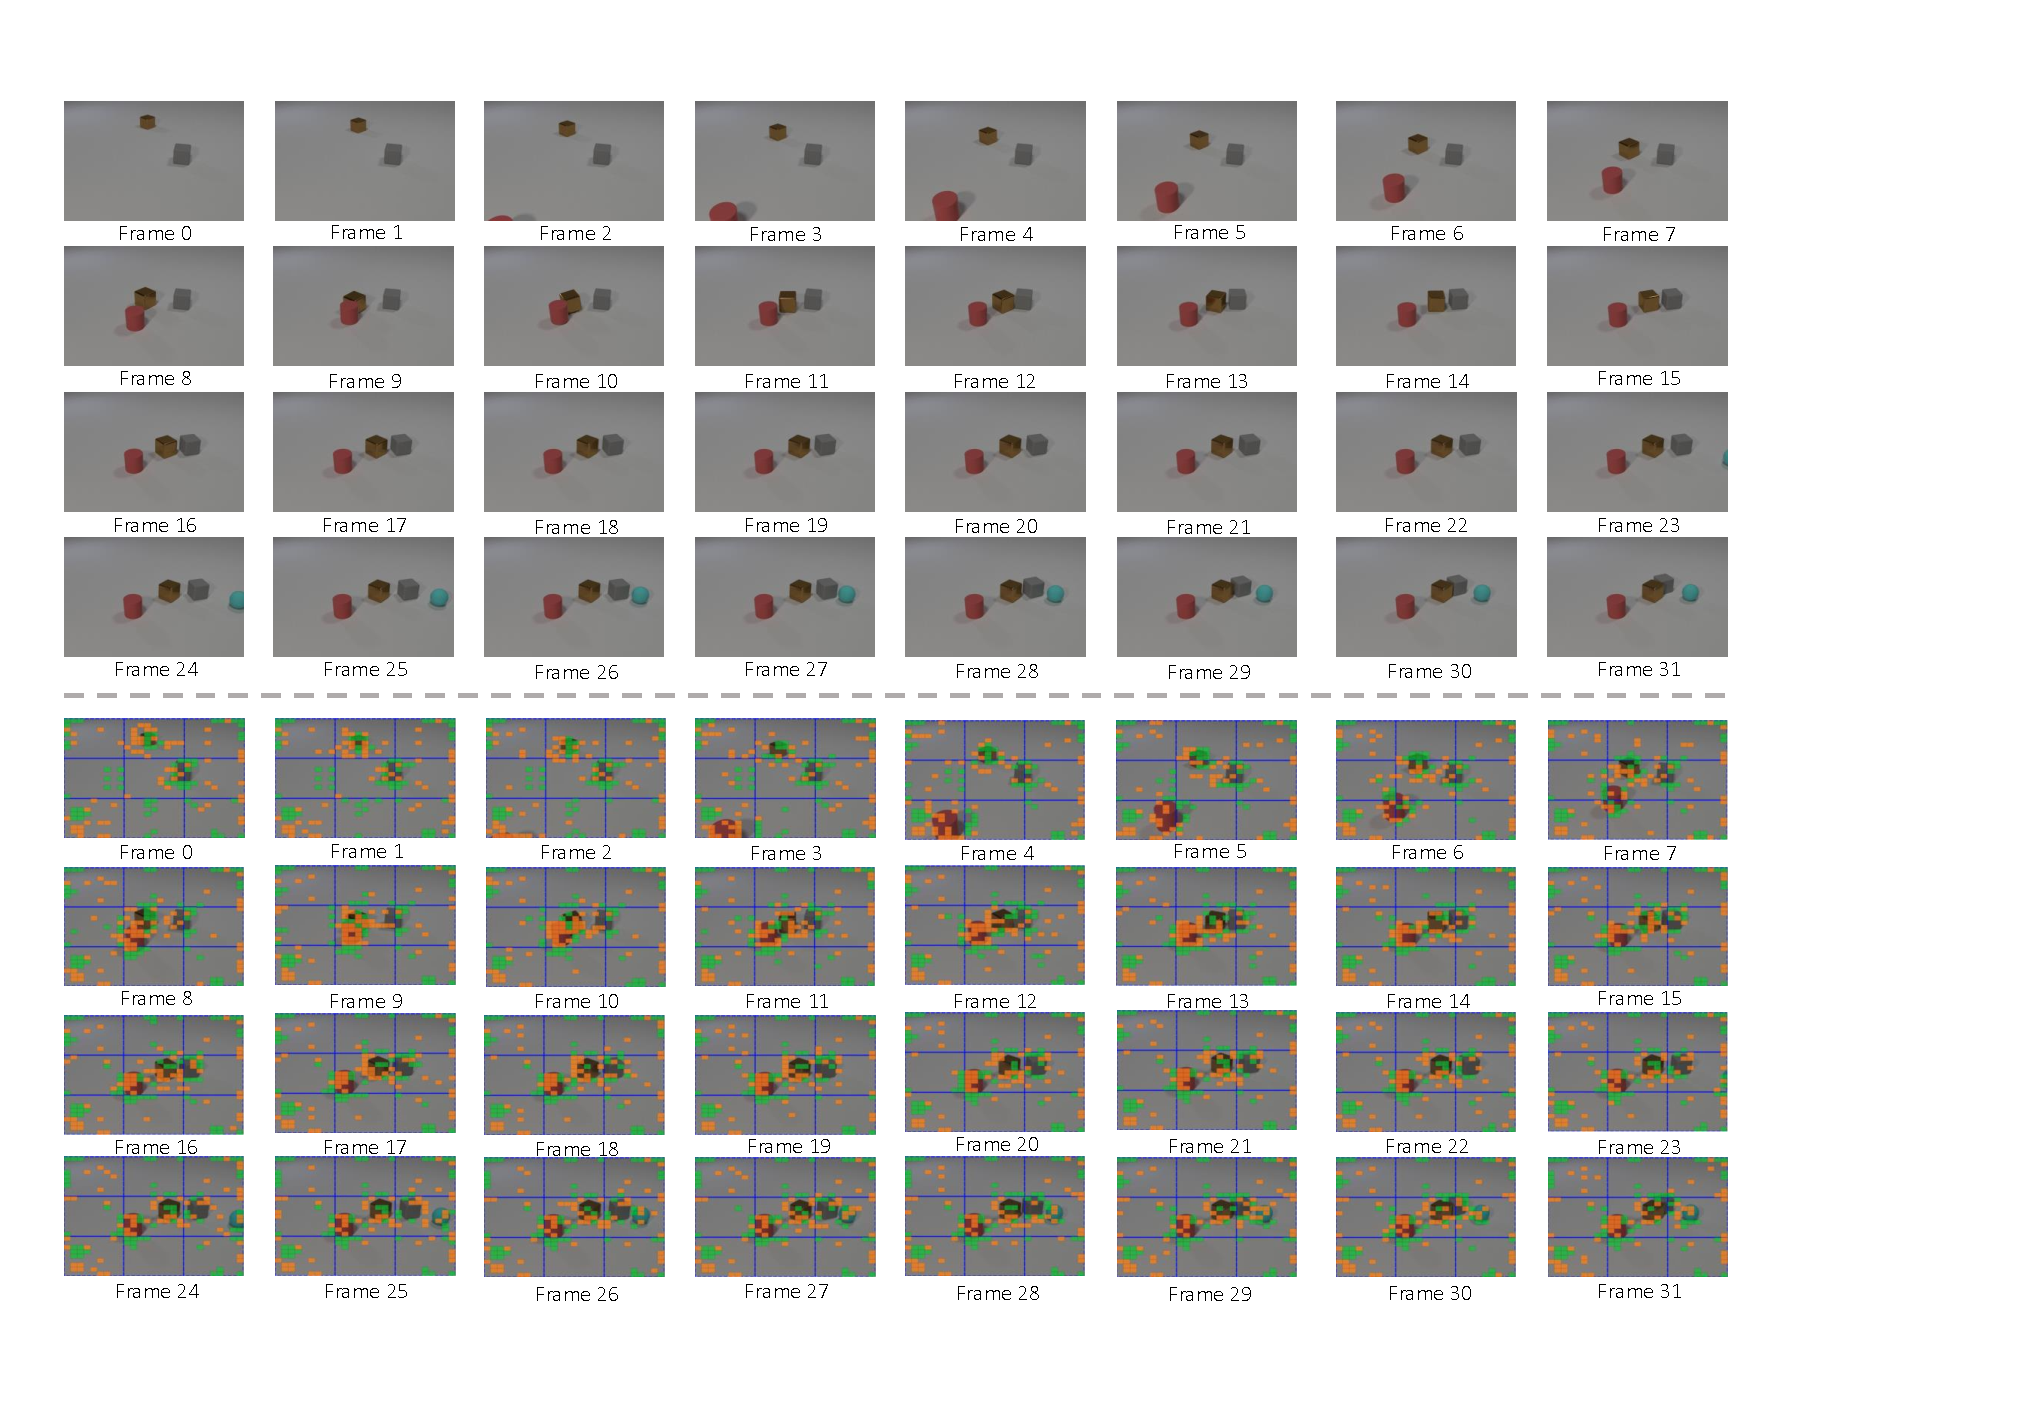
\includegraphics[width=\linewidth]{figs/cvpr2026_supple_vis_01.pdf}
    % \vspace{-0.8cm}
    \caption{Qualitative visualizations of our \textcolor{green}{Local}-\textcolor{orange}{Global} token anchors evolution across consecutive frames on MVBench sample while optimal transport is adopted to aggregate necessary information from unselected tokens to help LLM precess better. The top is the original sampled frames while the bottom is the corresponding tokens visualization.}
\label{fig:supple_vis_01}
% \vspace{-0.4cm}
\end{figure*}


\begin{figure*}[t]
    \centering
    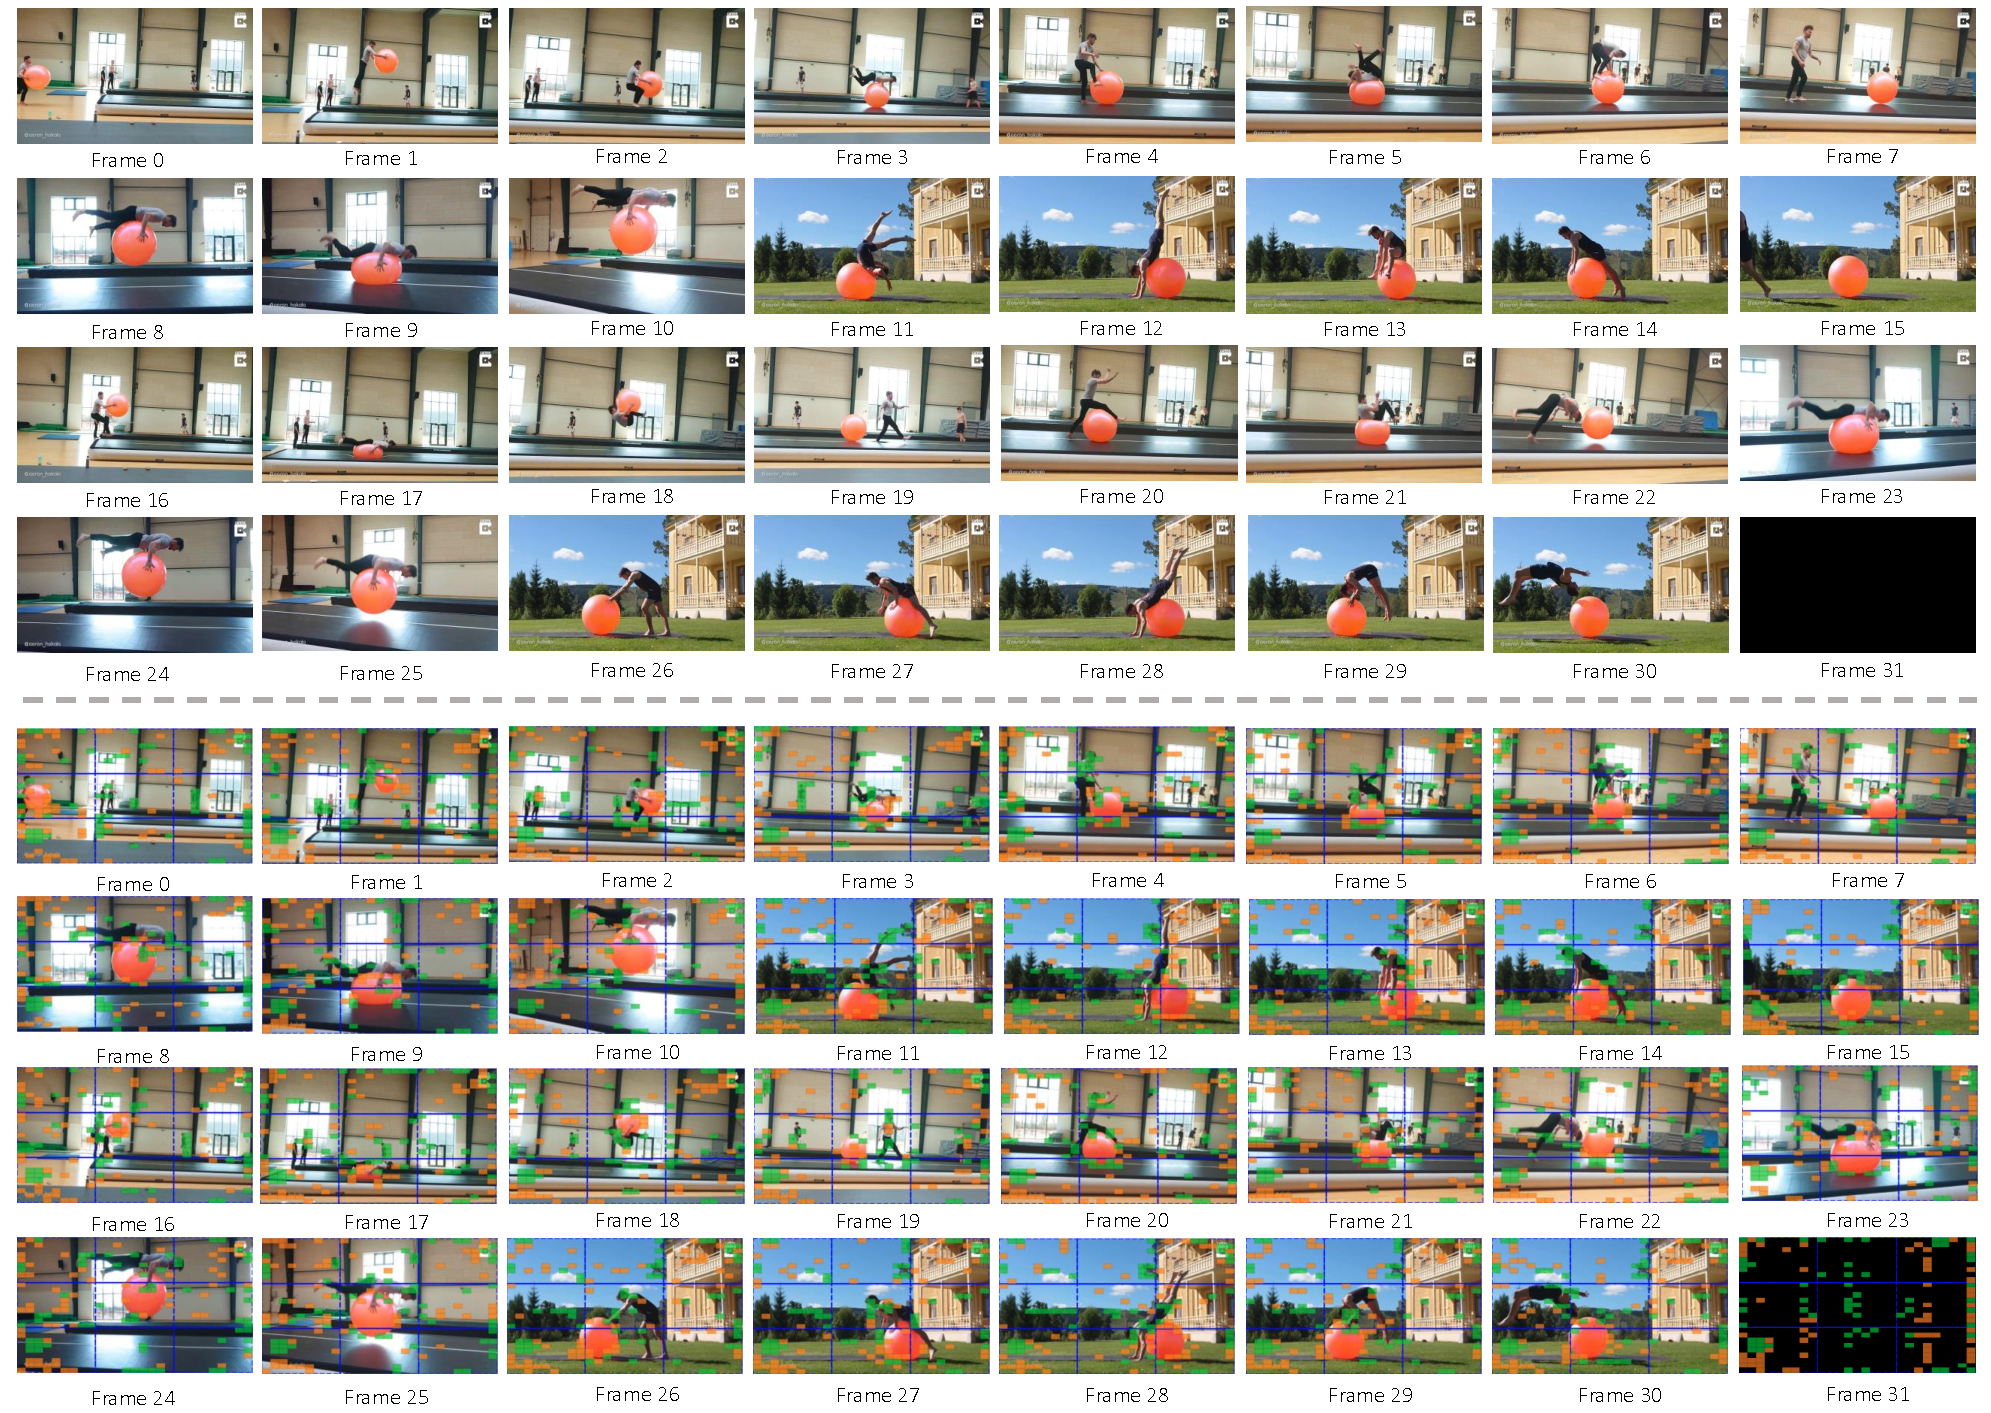
\includegraphics[width=\linewidth]{figs/cvpr2026_supple_vis_02_cropped.pdf}
    % \vspace{-0.8cm}
    \caption{Qualitative visualizations of our \textcolor{green}{Local}-\textcolor{orange}{Global} token anchors evolution across consecutive frames on VideoMME sample while optimal transport is adopted to aggregate necessary information from unselected tokens to help LLM precess better. The top is the original sampled frames while the bottom is the corresponding tokens visualization.}
\label{fig:supple_vis_02}
% \vspace{-0.4cm}
\end{figure*}

\clearpage
\clearpage
